\documentclass[fleqn,10pt,serif,xcolor=dvipsnames]{beamer}

%========================================
% Packages
%========================================

\usepackage{etex}

\usepackage[palatino]{mypackBeamer}

\usepackage{gb4e_micha}

%========================================
% Commands
%========================================

\usepackage{mycommands}

%========================================
% More Layout (Beamer Special)
%========================================

\usetheme[height=0mm]{Rochester}
%\usetheme{Warsaw}


\usecolortheme{dove}

%\useoutertheme[footline=empty,compress,subsection=false]{miniframes}

\usecolortheme[named=Gray]{structure}

\setbeamercolor{title}{fg=Black}

%\setbeamercolor{structure}{fg=Brown}
%\setbeamercolor{normal text}{fg=Brown}
\setbeamercolor{section in head/foot}{bg=gray!20}
%\setbeamercolor{lower separation line head}{bg=black!40}
\setbeamercolor*{frametitle}{fg=Black,bg=gray!20}
\setbeamercolor*{block body}{fg=Black,bg=gray!00}
\setbeamercolor*{block title}{fg=Black,bg=gray!20}
 

% Switch of shadows of boxes
\setbeamertemplate{blocks}[default]

% Frame numbers in footer
\setbeamertemplate{footline}[frame number]

% See-through preview for uncovered
\setbeamercovered{transparent}

% Switch off navigation panel at bottom right
\beamertemplatenavigationsymbolsempty

% Change Style for itemize markers
% Options are ball, circle, rectangle and default (=triangle)
\setbeamertemplate{items}[circle] 

%\includeonlyframes{current}


\setcounter{tocdepth}{1}

% Use bullets in enumerates and TOC
\setbeamertemplate{enumerate item}[circle]

% Set color for enumerate/TOC bullets to white
\setbeamercolor*{item projected}{fg=Black,bg=gray!00}

%========================================
% Special this document
%========================================



%========================================
% Document
%========================================



\title{Processing of Scalar Items in Embedded Position}
\subtitle{An experimental study} 



\author{Petra Augurzky, Michael Franke \& Fabian Schlotterbeck}
\institute{Seminar f\"{u}r Sprachwissenschaft \& SFB~833 \\
  Eberhard Karls Universit\"{a}t T\"{u}bingen}
\date{}

% Logo auf allen Folien
% \logo{\pgfimage[height=2cm]{uni-tuebingen-logo.pdf}} 

% Logo auf Titelseite
\titlegraphic{\pgfimage[height=1.5cm]{unilogo.pdf}}

%--------------------------------------


\begin{document}

% --- Horizontal Space Fix ----

\abovedisplayskip=3pt 
\abovedisplayshortskip=3pt 

\belowdisplayskip=3pt 
\belowdisplayshortskip=3pt 


\begin{frame}[plain]
  \titlepage
\end{frame}

\begin{frame}
  \frametitle{Overview}
    \begin{enumerate}
    \item background \hfill (Michael)
    \item design \hfill (Petra)
    \item results \hfill (Fabian)
    \end{enumerate}
\end{frame}

\begin{frame}
  \frametitle{Scalar Implicatures}
  \begin{block}{Example}
    \begin{exe}
    \ex  \label{bsp:SI_Kiki_Target} Some of Kiki's friends are
      metalheads. \hfill (target)
    \ex  \label{bsp:SI_Kiki_Alternative_here} All of Kiki's friends
      are metalheads. \hfill (alternative)
    \ex It's not the case that all of Kiki's friends are
      \acros{mh}. \hfill (not-(\ref{bsp:SI_Kiki_Alternative_here}))
    \ex Some but not all of Kiki's friends are metalheads. \hfill ((1)
      \& (3))
    \end{exe}
  \end{block}
\end{frame}

\begin{frame}
  \frametitle{Scalar Implicatures}
  \begin{block}{Neo-Gricean Recipe}
    \begin{itemize}
    \item let $S(x)$ be a sentence in which scalar element $x$ occurs (once)
    \item let $\mathrm{Alt}(x)$ be a set of lexical alternatives to $x$
    \item let $S(y)$ be the sentence obtained by replacing $x$ in
      $S(x)$ with $y$
    \item[$\Rightarrow$] utterance of $S(x)$ implicates:
      \begin{center}
        it's not the case that $S(y)$\\
        (for all $y \in \mathrm{Alt}(x)$ such that
      $S(y)$ implicates $S(x)$)
      \end{center}
      
    \end{itemize}
  \end{block}
\end{frame}

\begin{frame}
  \frametitle{Scalar Items in Embedded Positions}
  \begin{block}{In upward monotonic position}
    \begin{exe}
    \ex \label{bsp:AE} All of the students read some of the papers.
    \end{exe}
  \end{block}
  \begin{block}{In non-monotonic position}
    \begin{exe}
    \ex \label{bsp:GE} Exactly one of the students read some of the papers.
    \end{exe}
  \end{block}
  % \bigskip
  % \begin{itemize}
  % \item[$\Rightarrow$] two kinds of pragmatic enrichment conceivable:
  % \item[(i)] global
  % \item[(ii)] local
  % \end{itemize}
\end{frame}

\begin{frame}
  \frametitle{Scalar Items in Embedded Positions}
  \begin{block}{Global Enrichments}
    \dots see Neo-Gricean Recipe \dots
  \end{block}

  \begin{block}{Local Enrichments}
    \begin{itemize}
      \item $S(x)$ and $\mathtt{Alt}(x)$ as before
      \item write $x \& \neg y$ for composite element of same type as
        $x$
        \begin{itemize}
        \item[] e.g., ``some but not all''
        \end{itemize}
      \item[$\Rightarrow$] utterance of $S(x)$ implicates:
        \begin{center}
          $S(x \& \neg y)$\\
        (for all $y \in \mathtt{Alt}(x)$ such that ???)
        \end{center}
    \end{itemize}
  \end{block}
\end{frame}


\begin{frame}
  \frametitle{Scalar Items in Embedded Positions}
  \begin{block}{In upward monotonic position \hfill (Global)}
    \begin{exe}
      \exr{bsp:AE} All of the students read {\color{blue}{some}} of the
      papers.
    \ex All of the students read {\color{blue}{all}} of the papers.
    \ex
      \begin{xlist}
      \ex All of the students read some of the papers and  \\
        not all students read all
        of the papers.
      \ex All read some and at least one did not read all.
      \end{xlist}
    \end{exe}
  \end{block}
  \begin{block}{In upward monotonic position \hfill (Local)}
    \begin{exe}
      \exr{bsp:AE} All of the students read {\color{blue}{some}} of the
      papers.
    \ex
      \begin{xlist}
      \ex All of the students read {\color{blue}{some  but not all}} of the papers.
      \ex All read some and no one read all.
      \end{xlist}
    \end{exe}
  \end{block}
\end{frame}


\begin{frame}
  \frametitle{Scalar Items in Embedded Positions}
  \begin{block}{In upward monotonic position}
    3 kinds of readings:
    \begin{enumerate}
    \item \textbf{literal}: all \dots some \dots
    \item \textbf{global}: all \dots some \dots \& not (all \dots all \dots)
    \item \textbf{local}: all \dots some but not all \dots
    \end{enumerate}
    with entailment relations:
    \begin{itemize}
    \item[] \acro{lit} $\supset$ \acro{glb} $\supset$ \acro{loc}
    \end{itemize}
  \end{block}
\end{frame}

\begin{frame}
  \frametitle{Scalar Items in Embedded Positions}
  \begin{block}{In upward monotonic position \hfill (Entailment Relations)}
    
    \medskip 

    \begin{minipage}[c]{0.5\linewidth}
      \vspace{0pt}
      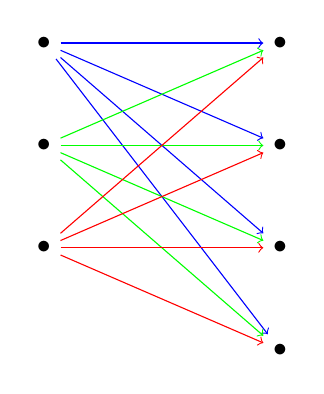
\begin{tikzpicture}[node distance = 1.3cm]
        % Nodes

        \node (X-1) {$\Large{\bullet}$};

        \node (X-2) [below of = X-1] {$\Large{\bullet}$};

        \node (X-3) [below of = X-2] {$\Large{\bullet}$};

        \node (Y-1) [right of = X-1, node distance = 3cm]{$\Large{\bullet}$};

        \node (Y-2) [below of = Y-1] {$\Large{\bullet}$};

        \node (Y-3) [below of = Y-2] {$\Large{\bullet}$};

        \node (Y-4) [below of = Y-3] {$\Large{\bullet}$};

        % Arrows

        \path [draw=blue,->] (X-1) -> (Y-1);

        \path [draw=blue,->] (X-1) -> (Y-2);

        \path [draw=blue,->] (X-1) -> (Y-3);

        \path [draw=blue,->] (X-1) -> (Y-4);


        \path [draw=green,->] (X-2) -> (Y-1);

        \path [draw=green,->] (X-2) -> (Y-2);

        \path [draw=green,->] (X-2) -> (Y-3);

        \path [draw=green,->] (X-2) -> (Y-4);



        \path [draw=red,->] (X-3) -> (Y-1);

        \path [draw=red,->] (X-3) -> (Y-2);

        \path [draw=red,->] (X-3) -> (Y-3);

        \path [draw=red,->] (X-3) -> (Y-4);

      \end{tikzpicture}
      \end{minipage}
      \begin{minipage}[c]{0.45\linewidth}
        \vspace{0pt}
    ``All of the dots on the left are connected to some of the dots on
    the right.''
    \medskip

        \begin{itemize}
        \item[] \acro{lit}: True
        \item[] \acro{glb}: False
        \item[] \acro{loc}: False 
        \end{itemize}
      \end{minipage}

  \end{block}
\end{frame}

\begin{frame}
  \frametitle{Scalar Items in Embedded Positions}
  \begin{block}{In upward monotonic position \hfill (Entailment Relations)}
    
    \medskip 

    \begin{minipage}[c]{0.5\linewidth}
      \vspace{0pt}
            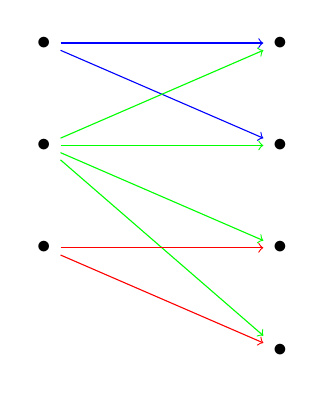
\begin{tikzpicture}[node distance = 1.3cm]
        % Nodes

        \node (X-1) {$\Large{\bullet}$};

        \node (X-2) [below of = X-1] {$\Large{\bullet}$};

        \node (X-3) [below of = X-2] {$\Large{\bullet}$};

        \node (Y-1) [right of = X-1, node distance = 3cm]{$\Large{\bullet}$};

        \node (Y-2) [below of = Y-1] {$\Large{\bullet}$};

        \node (Y-3) [below of = Y-2] {$\Large{\bullet}$};

        \node (Y-4) [below of = Y-3] {$\Large{\bullet}$};

        % Arrows

        \path [draw=blue,->] (X-1) -> (Y-1);

        \path [draw=blue,->] (X-1) -> (Y-2);


        \path [draw=green,->] (X-2) -> (Y-1);

        \path [draw=green,->] (X-2) -> (Y-2);

        \path [draw=green,->] (X-2) -> (Y-3);

        \path [draw=green,->] (X-2) -> (Y-4);


        \path [draw=red,->] (X-3) -> (Y-3);

        \path [draw=red,->] (X-3) -> (Y-4);

      \end{tikzpicture}
      \end{minipage}
      \begin{minipage}[c]{0.45\linewidth}
        \vspace{0pt}
    ``All of the dots on the left are connected to some of the dots on
    the right.''
    \medskip

        \begin{itemize}
        \item[] \acro{lit}: True
        \item[] \acro{glb}: True
        \item[] \acro{loc}: False 
        \end{itemize}
      \end{minipage}

  \end{block}
\end{frame}


\begin{frame}
  \frametitle{Scalar Items in Embedded Positions}
  \begin{block}{In upward monotonic position \hfill (Entailment Relations)}
    
    \medskip 

    \begin{minipage}[c]{0.5\linewidth}
      \vspace{0pt}
            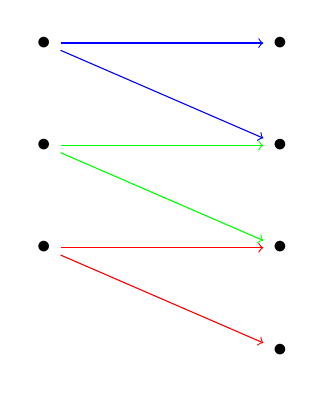
\begin{tikzpicture}[node distance = 1.3cm]
        % Nodes

        \node (X-1) {$\Large{\bullet}$};

        \node (X-2) [below of = X-1] {$\Large{\bullet}$};

        \node (X-3) [below of = X-2] {$\Large{\bullet}$};

        \node (Y-1) [right of = X-1, node distance = 3cm]{$\Large{\bullet}$};

        \node (Y-2) [below of = Y-1] {$\Large{\bullet}$};

        \node (Y-3) [below of = Y-2] {$\Large{\bullet}$};

        \node (Y-4) [below of = Y-3] {$\Large{\bullet}$};

        % Arrows

        \path [draw=blue,->] (X-1) -> (Y-1);

        \path [draw=blue,->] (X-1) -> (Y-2);


        \path [draw=green,->] (X-2) -> (Y-2);

        \path [draw=green,->] (X-2) -> (Y-3);


        \path [draw=red,->] (X-3) -> (Y-3);

        \path [draw=red,->] (X-3) -> (Y-4);

      \end{tikzpicture}
      \end{minipage}
      \begin{minipage}[c]{0.45\linewidth}
        \vspace{0pt}
    ``All of the dots on the left are connected to some of the dots on
    the right.''
    \medskip

        \begin{itemize}
        \item[] \acro{lit}: True
        \item[] \acro{glb}: True
        \item[] \acro{loc}: True 
        \end{itemize}
      \end{minipage}

  \end{block}
\end{frame}

%%%%%%%%%%%%%%%%%%%%%%%%%%%%%%%%%%%%%%%%%%%%%%%%%%
%%%%% Non-Monotonic
%%%%%%%%%%%%%%%%%%%%%%%%%%%%%%%%%%%%%%%%%%%%%%%%%%

\begin{frame}[shrink=2]
  \frametitle{Scalar Items in Embedded Positions}
  \begin{block}{In non-monotonic position \hfill (Global)}
    \begin{exe}
      \exr{bsp:GE} Exactly one of the students read {\color{blue}{some}} of the
      papers.
    \ex Exactly one of the students read {\color{blue}{all}} of the papers.
    \ex
      \begin{xlist}
      \ex Exactly one of the students read some and  \\
        it's not the case that exactly one read all.
      \ex Exactly one student read some but not all and  \\
        no one else read anything.
      \end{xlist}
    \end{exe}
  \end{block}
  \begin{block}{In upward monotonic position \hfill (Local)}
    \begin{exe}
      \exr{bsp:GE} Exactly one of the students read {\color{blue}{some}} of the
      papers.
    \ex
      \begin{xlist}
      \ex Exactly one of the students read {\color{blue}{some but not all}} of the papers.
      \ex Exactly one student read some but not all and  \\
        all of the others read all or nothing.
      \end{xlist}
    \end{exe}
  \end{block}
\end{frame}


\begin{frame}
  \frametitle{Scalar Items in Embedded Positions}
  \begin{block}{In non-monotonic position}
    3 kinds of readings:
    \begin{enumerate}
    \item \textbf{literal}: exactly one \dots some \dots
    \item \textbf{global}: exactly one \dots some \dots \& not (exactly one \dots all \dots)
    \item \textbf{local}: exactly one \dots some but not all \dots
    \end{enumerate}
    with entailment relations:
    \begin{itemize}
    \item[] \acro{lit} $\supset$ \acro{glb} $\color{blue}{\subset}$ \acro{loc}
    \item[] \acro{lit} $\not \supset$ \acro{loc}
    \end{itemize}
  \end{block}
\end{frame}

\begin{frame}
  \frametitle{Scalar Items in Embedded Positions}
  \begin{block}{In upward monotonic position \hfill (Entailment Relations)}
    
    \medskip 

    \begin{minipage}[c]{0.5\linewidth}
      \vspace{0pt}
      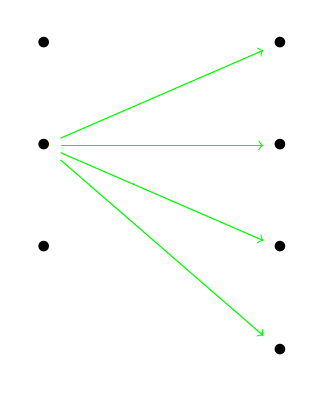
\begin{tikzpicture}[node distance = 1.3cm]
        % Nodes

        \node (X-1) {$\Large{\bullet}$};

        \node (X-2) [below of = X-1] {$\Large{\bullet}$};

        \node (X-3) [below of = X-2] {$\Large{\bullet}$};

        \node (Y-1) [right of = X-1, node distance = 3cm]{$\Large{\bullet}$};

        \node (Y-2) [below of = Y-1] {$\Large{\bullet}$};

        \node (Y-3) [below of = Y-2] {$\Large{\bullet}$};

        \node (Y-4) [below of = Y-3] {$\Large{\bullet}$};

        % Arrows

        \path [draw=green,->] (X-2) -> (Y-1);

        \path [draw=green,->] (X-2) -> (Y-2);

        \path [draw=green,->] (X-2) -> (Y-3);

        \path [draw=green,->] (X-2) -> (Y-4);

      \end{tikzpicture}
      \end{minipage}
      \begin{minipage}[c]{0.45\linewidth}
        \vspace{0pt}
    ``Exactly one of the dots on the left are connected to some of the dots on
    the right.''
    \medskip

        \begin{itemize}
        \item[] \acro{lit}: True
        \item[] \acro{glb}: False
        \item[] \acro{loc}: False 
        \end{itemize}
      \end{minipage}

  \end{block}
\end{frame}

\begin{frame}
  \frametitle{Scalar Items in Embedded Positions}
  \begin{block}{In upward monotonic position \hfill (Entailment Relations)}
    
    \medskip 

    \begin{minipage}[c]{0.5\linewidth}
      \vspace{0pt}
            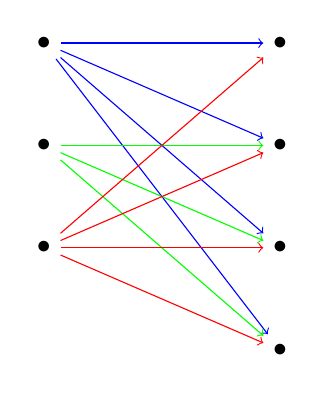
\begin{tikzpicture}[node distance = 1.3cm]
        % Nodes

        \node (X-1) {$\Large{\bullet}$};

        \node (X-2) [below of = X-1] {$\Large{\bullet}$};

        \node (X-3) [below of = X-2] {$\Large{\bullet}$};

        \node (Y-1) [right of = X-1, node distance = 3cm]{$\Large{\bullet}$};

        \node (Y-2) [below of = Y-1] {$\Large{\bullet}$};

        \node (Y-3) [below of = Y-2] {$\Large{\bullet}$};

        \node (Y-4) [below of = Y-3] {$\Large{\bullet}$};

        % Arrows

        \path [draw=blue,->] (X-1) -> (Y-1);

        \path [draw=blue,->] (X-1) -> (Y-2);

        \path [draw=blue,->] (X-1) -> (Y-3);

        \path [draw=blue,->] (X-1) -> (Y-4);



        \path [draw=green,->] (X-2) -> (Y-2);

        \path [draw=green,->] (X-2) -> (Y-3);

        \path [draw=green,->] (X-2) -> (Y-4);



        \path [draw=red,->] (X-3) -> (Y-1);

        \path [draw=red,->] (X-3) -> (Y-2);

        \path [draw=red,->] (X-3) -> (Y-3);

        \path [draw=red,->] (X-3) -> (Y-4);

      \end{tikzpicture}
      \end{minipage}
      \begin{minipage}[c]{0.45\linewidth}
        \vspace{0pt}
    ``All of the dots on the left are connected to some of the dots on
    the right.''
    \medskip

        \begin{itemize}
        \item[] \acro{lit}: False
        \item[] \acro{glb}: False
        \item[] \acro{loc}: True 
        \end{itemize}
      \end{minipage}

  \end{block}
\end{frame}


\begin{frame}
  \frametitle{Scalar Items in Embedded Positions}
  \begin{block}{In upward monotonic position \hfill (Entailment Relations)}
    
    \medskip 

    \begin{minipage}[c]{0.5\linewidth}
      \vspace{0pt}
      \begin{tikzpicture}[node distance = 1.3cm]
        % Nodes

        \node (X-1) {$\Large{\bullet}$};

        \node (X-2) [below of = X-1] {$\Large{\bullet}$};

        \node (X-3) [below of = X-2] {$\Large{\bullet}$};

        \node (Y-1) [right of = X-1, node distance = 3cm]{$\Large{\bullet}$};

        \node (Y-2) [below of = Y-1] {$\Large{\bullet}$};

        \node (Y-3) [below of = Y-2] {$\Large{\bullet}$};

        \node (Y-4) [below of = Y-3] {$\Large{\bullet}$};

        % Arrows

        \path [draw=blue,->] (X-1) -> (Y-1);

        \path [draw=blue,->] (X-1) -> (Y-2);

      \end{tikzpicture}
      \end{minipage}
      \begin{minipage}[c]{0.45\linewidth}
        \vspace{0pt}
    ``All of the dots on the left are connected to some of the dots on
    the right.''
    \medskip

        \begin{itemize}
        \item[] \acro{lit}: True
        \item[] \acro{glb}: True
        \item[] \acro{loc}: True 
        \end{itemize}
      \end{minipage}

  \end{block}
\end{frame}

\begin{frame}
  \frametitle{Experimental Study 1:
    \citet{GeurtsPouscoulous2009:Embedded-Implic}}
  \begin{minipage}[t]{0.6\linewidth}
    \vspace{0cm}
      \begin{itemize}
      \item picture verification task
      \item critical sentences:
        \begin{enumerate}
        \item[AE] All the squares are connected with some of the
          circles. 
        \item[GE] Exactly two squares are connected with some of the
          circles. 
        \end{enumerate}
      \item critical pictures:
        \begin{enumerate}
        \item[AE] true for \acro{lit} and \acro{glb}; false for \acro{loc}
        \item[GE] true for \acro{loc}; false for \acro{lit} and \acro{glb} 
        \end{enumerate}
      \item results: no \acro{loc}-responses \emph{at all}!
      \end{itemize}
  \end{minipage}
  \hspace{0.1cm}
  \begin{minipage}[t]{0.35\linewidth}
    \vspace{0cm}
    \begin{flushright}
      \includegraphics[scale=0.35]{Geurts_Pouscoulous_2009_ExpItem.png}
    \end{flushright}
  \end{minipage}
\end{frame}

\begin{frame}
  \frametitle{Experimental Study 2:
    \citet{ChemlaSpector2010:Experimental-Ev}}
  \begin{minipage}[t]{0.6\linewidth}
    \vspace{0cm}
      \begin{itemize}
      \item ``picture rating task'':
        \begin{itemize}
        \item continuous \acro{tv}-judgements
        \end{itemize}
      \item critical sentences:
        \begin{enumerate}
        \item[AE] Each letter is connected with some of its circles.
        \item[GE] Exactly one letter is connected with some of its circles. 
        \end{enumerate}
      \item critical pictures:
        \begin{enumerate}
        \item[AE] true for \acro{lit} and \acro{glb}; false for \acro{loc}
        \item[GE] true for \acro{loc}; false for \acro{lit} and \acro{glb} 
        \end{enumerate}
      \item results: attested \acro{loc}-responses!
      \end{itemize}
  \end{minipage}
  \hspace{0.1cm}
  \begin{minipage}[t]{0.35\linewidth}
    \vspace{0cm}
    \begin{center}
      \includegraphics[scale=0.25]{Chemla_Spector_2010_Critical_AE.png}\\
      \includegraphics[scale=0.25]{Chemla_Spector_2010_RatingBar.png}
    \end{center}
  \end{minipage}
\end{frame}

\begin{frame}
  \frametitle{Experimental Study 2:
    \citet{ChemlaSpector2010:Experimental-Ev}}
  \begin{block}{Results \acro{ae}}
    \medskip
    \includegraphics[width=6.5cm]{Chemla_Spector_2010_ExpItem.png}
    \includegraphics[width=4.5cm]{Chemla_Spector_2010_Results_AE.png}
    \medskip
    \begin{center}
      ``Each letter is connected to some of its circles.''
    \end{center}
  \end{block}
\end{frame}


\begin{frame}
  \frametitle{Experimental Study 2:
    \citet{ChemlaSpector2010:Experimental-Ev}}
  \begin{block}{Results \acro{ge}}
    \medskip
    \includegraphics[width=6.5cm]{Chemla_Spector_2010_ExpItem_GE.png}
    \includegraphics[width=4.5cm]{Chemla_Spector_2010_Results_GE.png}
    \medskip
    \begin{center}
      ``Exactly one letter is connected to some of its circles.''
    \end{center}
  \end{block}
\end{frame}

\begin{frame}
  \frametitle{Experimental Study 3: ``K1''}
  \begin{minipage}[t]{0.6\linewidth}
    \vspace{0cm}
      \begin{itemize}
      \item picture verification task
      \item critical sentences:
        \begin{enumerate}
        \item[AE] F\"{u}r jeden dieser Umweltsch\"{u}tzer gilt: er
          boykottierte einige dieser Gro\ss konzerne.
        \item[GE] F\"{u}r genau einen dieser Umweltsch\"{u}tzer gilt:
          er boykottierte einige dieser Gro\ss konzerne.
        \end{enumerate}
      \item critical pictures:
        \begin{enumerate}
        \item[AE] true for \acro{lit} and \acro{glb}; false for \acro{loc}
        \item[GE] true for \acro{loc}; false for \acro{lit} and \acro{glb} 
        \end{enumerate}
      \item results: attested \acro{loc}-responses
      \end{itemize}
  \end{minipage}
  \hspace{0.1cm}
  \begin{minipage}[t]{0.35\linewidth}
    \vspace{0cm}
    \begin{flushright}
      \includegraphics[width=3.8cm]{./../../pictures/Umweltschuetzer02.PNG}
      \vspace{-0.7cm}
      \begin{center}
        \acro{ae}-condition
      \end{center}
      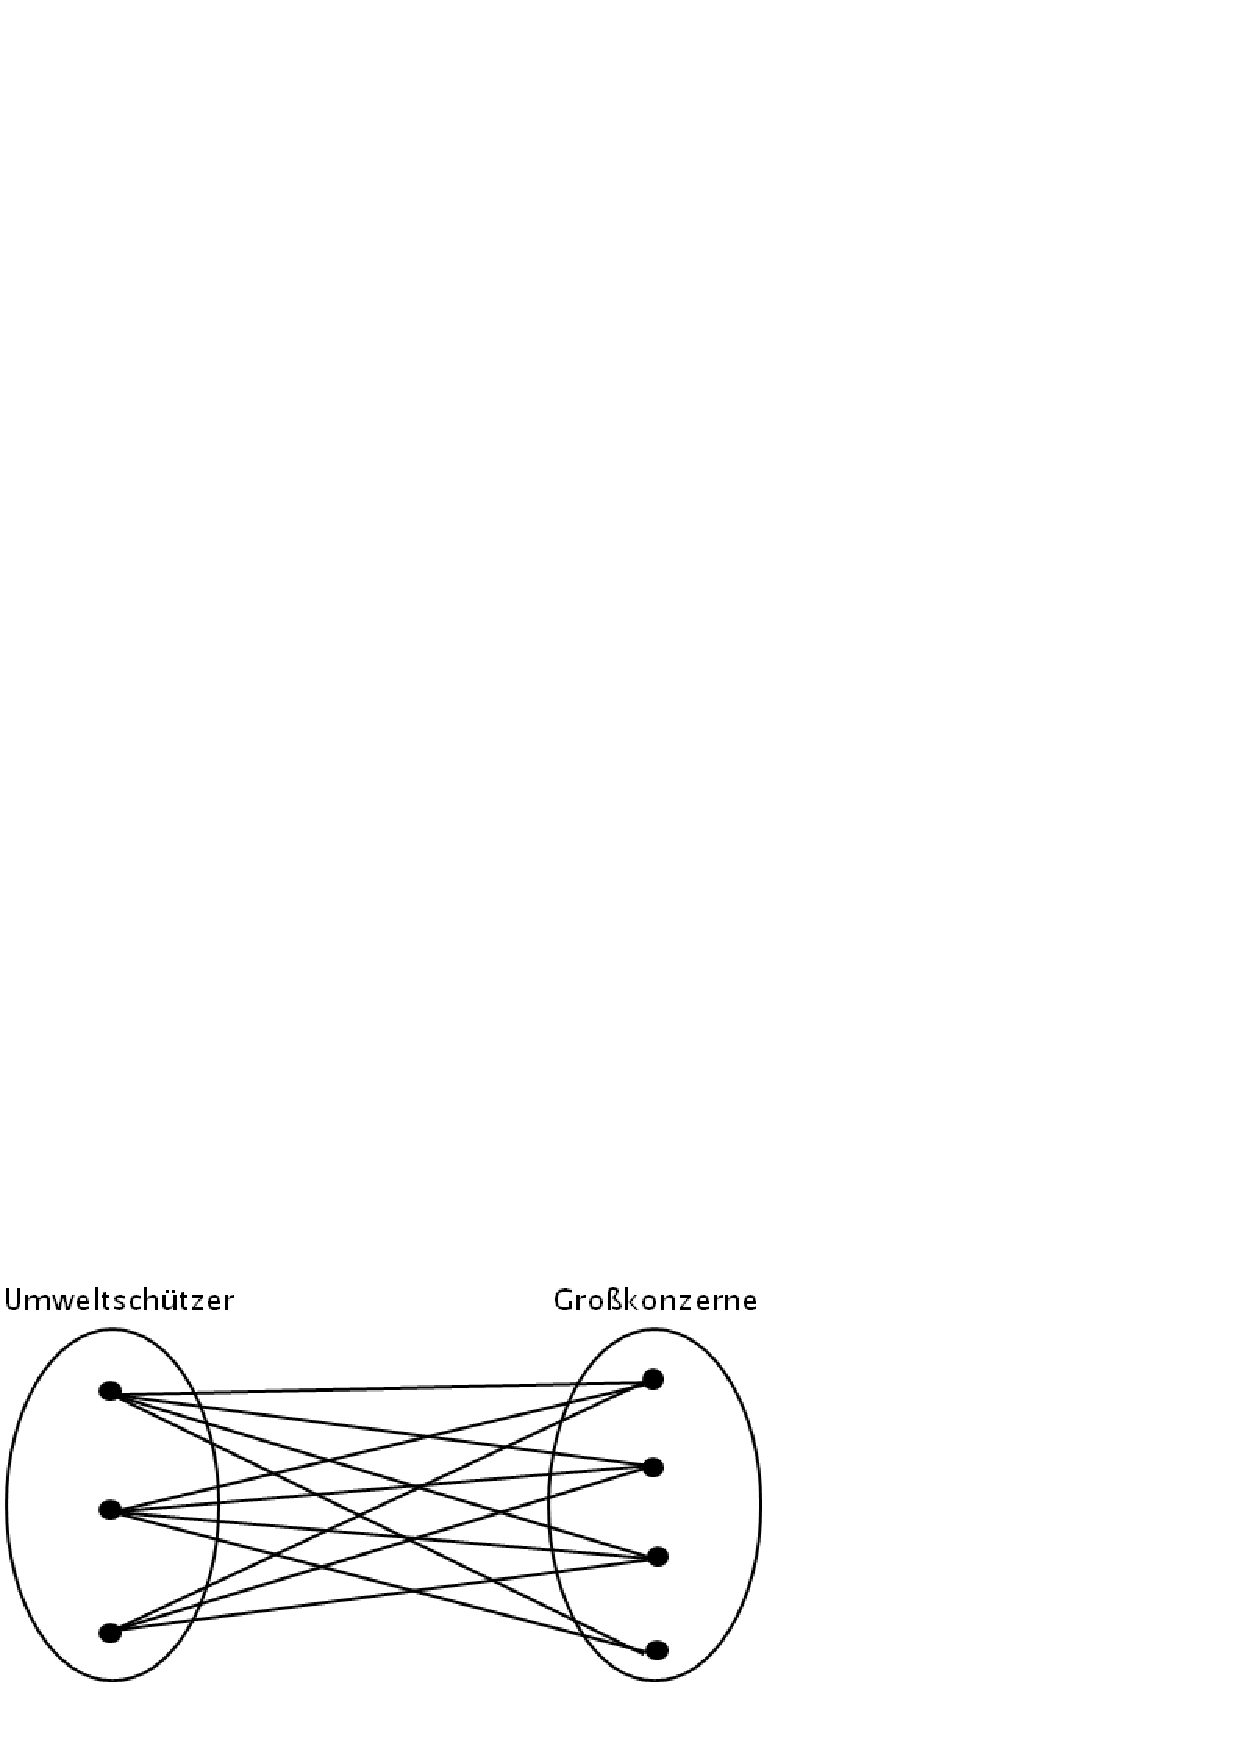
\includegraphics[width=4cm]{./../../pictures/Umweltschuetzer06.PNG}
      \vspace{-0.7cm}
      \begin{center}
        \acro{ge}-condition
      \end{center}
    \end{flushright}
  \end{minipage}
\end{frame}


\begin{frame}
  \frametitle{Experimental Study 3: ``K1''}
  \begin{block}{Results}
    \begin{minipage}[t]{0.45\linewidth}
      \vspace{0cm}
      \includegraphics[scale=0.3]{K1_Results_AE.png}
      \vspace{-0.6cm}
      \begin{center}
        \acro{ae}-condition
      \end{center}
    \end{minipage}
    \hspace{0.3cm}
    \begin{minipage}[t]{0.45\linewidth}
      \vspace{0cm}
      \includegraphics[scale=0.3]{K1_Results_GE.png}
      \vspace{-0.6cm}
      \begin{center}
        \acro{ge}-condition
      \end{center}
    \end{minipage}
  \end{block}
\end{frame}




\begin{frame}[plain,allowframebreaks]
  \large{\textbf{References}}
    \printbibliography[heading=subbibliography]
\end{frame}
\end{document}



